\documentclass[oneside]{memoir}
\usepackage[utf8]{inputenc}
\usepackage[ngerman]{babel}
\usepackage[T1]{fontenc}
\usepackage{lettrine}
\usepackage{graphicx}
\DisemulatePackage{setspace}
\usepackage{setspace}
\onehalfspacing

\newcommand{\parasep}{
\bigskip
\bigskip
\begin{center} 
   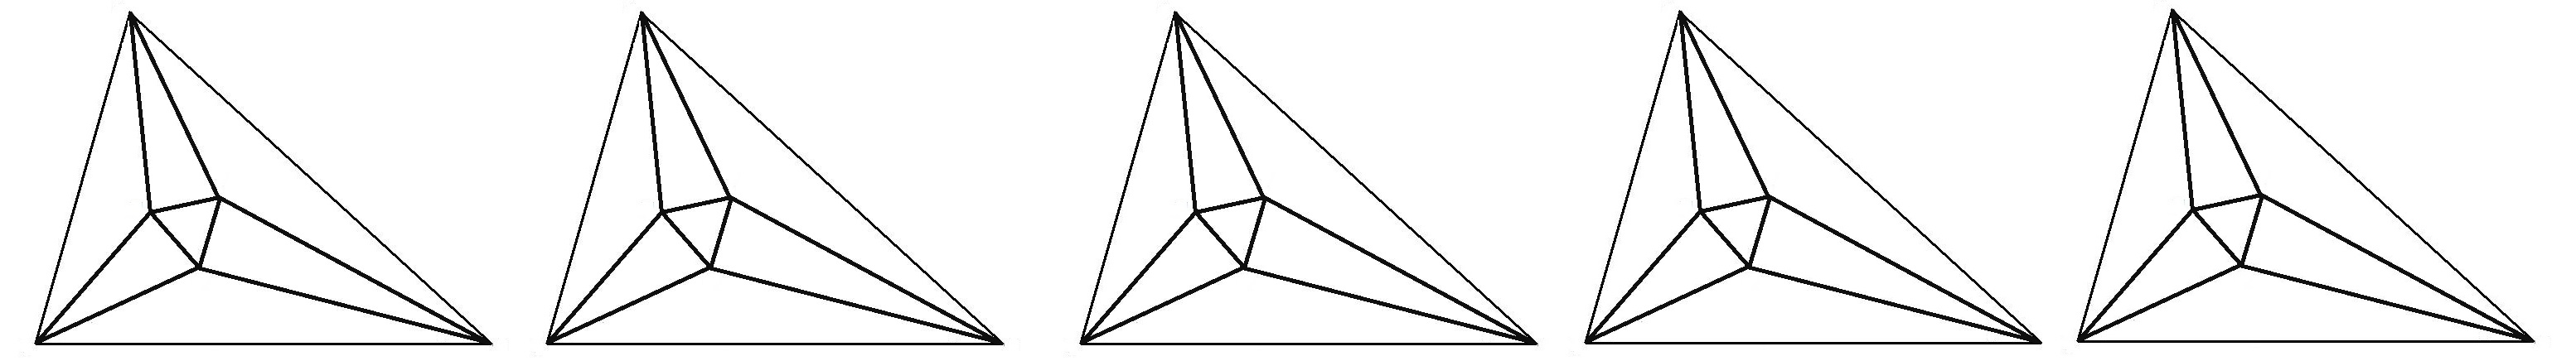
\includegraphics[scale=.08]{parasep5.jpg} 
\end{center}
\bigskip
\bigskip
}

\makeatletter
\newenvironment{chapquote}[2][2em]
  {\setlength{\@tempdima}{#1}%
   \def\chapquote@author{#2}%
   \parshape 1 \@tempdima \dimexpr\textwidth-2\@tempdima\relax%
   \itshape}
  {\par\normalfont\hfill--\ \chapquote@author\hspace*{\@tempdima}\par\bigskip}
\makeatother
\pretitle{\begin{center}\Huge\bfseries}
\title{In Jürgen's Keller}
\posttitle{\par\vskip1em{\normalfont\normalsize\scshape Eine AIMO-Geschichte\par\vfill}\end{center}}
\author{Herausgegeben von einer nichtleeren Teilmenge der AIMO-Teilnehmer 2020}
\predate{\vfill\begin{center}\large}
\begin{document}
\begin{titlingpage}
\maketitle
\end{titlingpage}
\chapter{Prolog in der Hölle}

\begin{chapquote}{Fyodor Dostoevsky}
\glqq Aus hundert Kaninchen wird niemals ein Pferd und aus hundert Verdachtsgründen niemals ein Beweis.\grqq
\end{chapquote}

\lettrine{M}{arc Hieke} schaute müde von den zahlreichen Mathematikaufgaben vor ihm wieder auf.

\chapter{Definitionen und Grundbegriffe} %bis 1.5
\begin{chapquote}{Veran Stojanović}
\glqq Was wir wissen, ein Epsilon. Was wir nicht wissen, ein 1/Epsilon.\grqq
\end{chapquote}
\textit{Der 20. April 2020} \\ 
\lettrine{D}{ie Teilnehmerliste} auf der rechten Seite von Georgis Bildschirm füllte sich langsam, als Jürgen Prestin einen AIMO-Teilnehmer nach dem anderen in die Zoomsitzung ließ. Er gedachte, während dieser die am Abend davor abgeschickten Aufgaben zu besprechen. Die ihm inzwischen vertrauten Namen purzelten geradezu in die Sitzung, schon drei Minuten nach 16 Uhr waren so gut wie alle anwesend. Georgi nahm einen Schluck von der Tüte Orangensaft neben seinem Laptop und setzte seine Kopfhörer auf. Veran, Christian und Patrick waren bereits auf einem separaten Discordserver, in dem sie für gewöhnlich während den Seminaren ratschten – er beeilte sich und trat diesem bei. \\
„Und nach dem Eisensteinkriterium ist P irreduzibel, glaube ich“, beendete Christian seinen Gedanken, woraufhin Veran zögernd sein Einverständnis gab. \\
„Hi“, sagte Georgi und erhielt einen Gruß von den beiden anderen. „Wo ist Patrick?“ \\
„Unklar“, antwortete Veran schroff. „Wahrscheinlich spielt er gerade GTA oder so.“
Ein Rauschen war von Patricks Mikrofon zu hören. Vermutlich hatte er sich gerade hingesetzt. \\ 
„Jungs, ich hab‘ mir grad so dick n Salat geholt“, gluckste Patrick vergnügt. „Meine Mutter hat wieder welche gekauft.“
Georgi wollte etwas dazu sagen, als sich Jürgen Prestin meldete. Er werde nun anfangen, ohne auf die Nachzügler zu warten. Es fehlte nur noch Marc, der schon die letzten paar Seminare hatte sausen lassen. Keiner der vieren wusste, ob er sich entschuldigt hatte oder warum genau er nicht erschien. Der Dozent fragte, wer denn zuerst eine Aufgabe vorstellen möchte, und während Georgi gerade darüber nachdachte, ob er die zwei Aufgaben, die er vorbereitet hatte, jetzt oder später vorstellen wollte, klinkte sich Christian aus dem Discord aus, hob auf Zoom seine Stummschaltung auf und fing an, über die 5 zu referieren. 
Nachdem er fertig war, trat er dem Channel mit den anderen wieder bei.  \\
„Voll kreativ“, lobte ihn Veran, worauf Christian sich bedankte. Er fragte daraufhin die anderen beiden im Call, ob sie die Aufgabe ähnlich gelöst hatten. \\
„Bruder, ich hab‘ grad gar nicht aufgepasst“, erwiderte Patrick leicht aufgebracht. „Es hat mich wieder dieser komische Typ angerufen.“ \\
„Der Nummernachbar?“, fragte Georgi. Der Unbekannte mit derselben Nummer wie Patrick bis auf die letzte Ziffer hatte ihn bereits vor dem ersten Bad Homburg-Seminar kontaktiert und hatte nur wirres Zeug von sich gegeben. Obwohl Sofia und die anderen sich über Michael, so hatte er sich genannt, lustig machten, war er Patrick ganz und gar nicht geheuer. \\
„Ja“, antwortete Patrick. „Er war aufgeregt und hat irgendwas davon geredet, dass ich vorsichtig sein sollte. Ich hab‘ einfach aufgelegt, ich fand das zu seltsam.“ \\
„Fishy“, sagte Christian. „Ich glaube, du brauchst das nicht allzu ernst nehmen.“ \\
„Ja, glaub ich auch nicht.“, meinte Patrick und richtete seine Aufmerksamkeit auf seinen Salat. „Der Typ ist sowieso nicht ganz klar im Kopf.“

%1.2.
\parasep

\textit{Der 21. April 2020} \\ 
„Der Nummernnachbar von Patrick hat sich übrigens wieder gemeldet.“ Georgi telefonierte gerade mit seinem Freund Maximilian Keßler, welcher in den zwei Jahren zuvor an der AIMO teilgenommen und es 2019 auch zur IMO geschafft hatte, und berichtete ihm eifrig über die neuesten Geschehnisse. \\
 „Oh echt? Ich dachte der hat längst aufgehört, Patrick zu schreiben?“, wunderte sich Max. \\
 „Ja, das letzte Mal haben wir in Bad Homburg von ihm gehört. Aber gestern während dem AIMO-Meeting hat er wieder bei Patrick angerufen...“ Georgi erzählte ihm also alles über den mysteriösen Anruf. \\
 „Eure AIMO ist echt witzig, so etwas ist letztes und vorletztes Jahr nicht passiert!“, meinte Max Keßler daraufhin amüsiert. \\
 „Ja, das stimmt“, fand auch Georgi, „Aber dafür konntest du immerhin zu den Seminaren in Reallife fahren... \\
  „Oh ja, vor allem die Woche in Oberwolfach hätte ich dir auch gegönnt!“ \\
   „Jaa, Corona ist echt so eine Bitch.“ \\
    „Ich sag mal so, is nicht schön, aber wat willste machen?“, scherzte Max daraufhin und beide schmunzelten. Georgi erzählte weiter: \\
    „Aber mal im Ernst, die Zoom-Meetings sind einfach nicht das gleiche Erlebnis. Ich würde mich so langweilen, wenn ich nicht währenddessen mit den anderen über Discord reden würde. Marc zum Beispiel kommt seit einigen Tagen gar nicht mehr zu den Seminaren...“ \\
    „Marc Hieke?“, fragte Max nach. \\
     „Ja“, bestätigte Georgi. \\
     „Fishy. Gerade der sollte sich doch mal bisschen mehr anstrengen. Seine Platzierung auf der Schätzliste sieht im Moment gar nicht gut aus“, bemerkte Max. Georgi stimmte ihm zu, und nach einigen weiteren Diskussionen über die Schätzliste und die Seminare klopfte es an Georgis Tür und man hörte seine Mutter rufen: „Essen ist fertig!“ \\
     „Ah, ich muss dann wohl gehen“, sagte Georgi zu Max. \\
     „Dann guten Appetit!“, antwortete Max und die beiden verabschiedeten sich.
     
     \parasep
     %1.5
     \textit{Der 24. April 2020} \\ 
     
     Unter dem blauroten Licht der großen Serbienfahne, die über dem Bett in Sofias Zimmer hing, hörte man ein lautes, verstörendes Lachen, das die im Nebenzimmer schlafende Mutter aufweckte. Sie dachte, ihre Tochter sei verrückt, allein wegen der Tatsache, dass ihr Zimmer von lauter “Serbien” nicht atmen konnte. In Sofias Zimmer gab es nämlich, neben ihrem Lieblingskleid - der serbischen Nationaltracht - sowie der Flasche mit 89 \% igem echten serbischen Pflaumenschnaps, tausende - teilweise sehr nationalistische - Bilder, die Symbole, Sprüche, Gegenstände aus und über Serbien beinhalteten und Sofia so sehr faszinierten. Ihr dortiger Aufenthalt im Jahr zuvor hat in ihr eine enorme Begeisterung für das Land ausgelöst - sie werde eines Tages dort wohnen, sagte sie immer.  \\  \\ 

Auch in ihrem Telefonat mit Maria durften Serbienandeutungen nicht fehlen. Es war die Rede von einem “allgemeinen Beispiel” sowie von einer ominösen “Person A”. Dabei wollte Maria nur wissen, welchen Zug Sofia für das Seminar in Oberwolfach nimmt...  \\ 
“Ich nehm den um 08:49. Dann musst du aber sehr früh aufstehen...”.  \\ 
“Kein Problem” antwortete Maria; “Ich wach jeden Tag um Viertel vor sechs auf”. \\  
“Du könntest aber auch die Nacht davor bei mir übernachten, meine Mutter hätte nichts dagegen” schlug Sofia vor.  \\ 
“Hmm ich bin mir nicht sicher...” sagte Maria; “meine Mutter ist grad nicht da...”.  \\ 
“Du kannst doch deinen Vater fragen” fiel Sofia ein. 
Doch Maria reagierte darauf sehr zögernd, und Sofia verstand sofort, dass es ein Fehler war, das gesagt zu haben. \\ 
“Ich habe keinen Vater” erklärte Maria; “ich hab ihn seit meiner Geburt nie kennengelernt...und meine Mutter wollte nie darüber mit mir sprechen”. “Fishy” sagte Sofia darauf. 
Es folgten paar Sekunden Stille. 
 \\ 
“Ich bring Marzipan zum Seminar mit”  sagte Maria, um vom Thema abzulenken. 
“Jaaa” jubelte Sofia.  \\ 
“Wobei...fuck! Jebote! Marzipan beginnt mit M!”.  \\ 
“Und das heißt...?” reagierte Maria verwirrt.  \\ 
“Alle schlechten Dinge beginnen mit M!” antwortete Sofia voller Euphorie; “Das ist Teil von meiner neuen Lebenseinstellung! Aber keine Sorge, du beginnst nicht mit M, weil Maria Matthis hat ja zwei M, und das hebt sich auf”.  \\ 
“Ah ja” antwortete Maria und war noch einmal verstört von Sofias seltsamen Aussagen.  \\ 
“Ne Spaß ich mag Marzipan” beruhigte sie Sofia, nachdem sie gemerkt hatte, dass sie mal wieder etwas übertrieben hat.
“Sorry, ich glaub ich hab wieder zu viel Tee gegessen”.

Ab dem Moment wusste keiner mehr, was er sagen sollte.  \\ 
“Ich denke, ich muss jetzt schlafen gehen” entschloss sich Maria.
“Oke...” sagte Sofia, “Gute Nacht”. \\ 
“Gute Nacht” sagte auch Maria und stürzte sich ins Bett. 
Es erwarteten sie wieder aufregende Träume.
     
     \parasep
     %1.3
     \textit{Der 25. April 2020} \\
     
     Christian erwachte aus unruhigen Träumen. Wie immer, ließ er sich davon aber nicht ablenken und als die ersten paar Strahlen der Münchner Sonne in sein Gesicht schienen, wurde ihm sofort klar: Es ist ein perfekter Tag zum Baden!
So verlor er keine einzige Sekunde und führte in größter Eile seine gewöhnliche Morgenroutine durch.
Nachdem er dann schnell aber sorgfältig seine Zähne geputzt, geduscht, seine Badesachen angezogen, sich eingecremt (obwohl es draußen nur 20 Grad heiß war), dann mit seiner Familie nach einem kurzen Gebet ein paar Semmeln und Brezn gefrühstückt und danach kurz den “QED-Chat” gecheckt hatte, begab er sich auf eine wilde Fahrt zum Englischen Garten.
Er fuhr blitzschnell durch die Straßen von Schwabing, überquerte die Leopoldstraße und ließ sich dabei nicht von den Menschenmengen ablenken, die den schönen Tag in der Münchner Innenstadt verbringen wollten. Als er dann am großen Park ankam, wurde es schon etwas unangenehm, und das Fahrradfahren durch die mit Fußgängern gefüllten Wege war fast unmöglich. Obwohl dies für Christian eigentlich kein Problem darstellte, beschloss er diesmal, einen Umweg zu fahren - bis zum Eisbach war es schließlich nicht mehr so weit.
Er fuhr dann Richtung Norden und entdeckte Teile des Parks, in denen er noch nie gewesen war. Die Bäume wurden immer dichter und der Himmel bewölkter. Christian bekam langsam Zweifel, ob der Weg, den er fuhr, sicher der Richtige sei, allerdings blieb er recht zuversichtlich - den großen Eisbach könne er schließlich nicht verpassen.
Nach einigen Metern merkte er aber, dass mit seinem Fahrrad irgendwas nicht stimmt. Es machte seltsame Geräusche und fuhr nur noch sehr langsam. Er beschloss, es zu schieben, bis er eine größere Straße erreichen würde. Doch die Wege wurden immer enger und Christian verlor seine Orientierung. Von anderen Menschen war mittlerweile nichts mehr zu sehen. Die ersten Regentropfen fingen an zu fallen.
Christian hatte keine Kraft mehr. Als dann eine Herde von Enten die Straße überquerte, wurde ihm der Weg komplett gesperrt.  \\
Christian blieb stehen.
Der Regen wurde immer stärker. \\
Und dann spürte er hinter seinem Rücken eine menschliche Gestalt, die ihm immer näher kam.
Er hörte eine bekannte Stimme. \\
“Guten Tag, Herr Noaghiu” sagte sie.
Christian erstarrte.
 

\chapter{Einleitende Überlegungen} %bis 1.9
\begin{chapquote}{Sören Kierkegaard}
\glqq Wie ist doch die ganze Natur so ominös! Voll Vorbedeutung ist mir der Vögel Flug, ihr Schrei, der Fische ausgelaßnes Schlagen gegen die Oberfläche des Wassers, ihr Verschwinden in der Tiefe, fernes Hundegebell, eines Wagens fernes Gerassel, Schritte, die von fernher widerhallen. Nicht sehe ich Gespenster in dieser nächtlichen Stunde, nicht sehe ich, was war, sondern das, was kommen wird.\grqq
\end{chapquote}

     
       \parasep
     %1.6
     \textit{Der 26. April 2020} \\ 
     
       \parasep
     %1.7
     \textit{Der 30. April 2020} \\
     
     Es war Dienstag, der 30. April 2020, der 42. Frühlingstag, und 12:36 am Nachmittag. Herr Prestin saß gedankenversunken an seinem Schreibtisch, seine Katze strich ihm um die Beine, und aus der Küche war leise das Radio zuhören, auf dem NDR-Info gerade von dem neuen Antikörpertest berichtete, der eine Genauigkeit von über 99 Prozent haben solle. Doch das interessierte Herrn Prestin nicht, denn neben dem Vorbereitungsmaterial für die Erstsemester befanden sich auf seinem Schreibtisch einige sehr staubige Dokumente, die er soeben aus dem Keller geholt hatte. Sie waren noch aus seiner eigenen Studienzeit, unter anderem gab es dort ein Photo, welches in mit seinem Kommilitonen und guten Freund Michael kurz vor dem Abschluss zeigt. Die Erinnerung stimmte Herrn Prestin sentimental. Nichtsdestotrotz musste er es jetzt zusammen mit den Aufzeichnungen zum Morley-Dreieck (kurioserweise enthielten diese neben normalen geometrischen Skizzen auch überraschend viele Abbildungen von Schaukeln und sogar eine Anleitung zu deren Aufbau) schreddern, bevor er die Überbleibsel eventuell noch verbrennen wollte. Doch plötzlich klingelte es an der Tür. Schnell räumte Herr Prestin die verräterischen Unterlagen beiseite, bevor er zur Tür eilte, doch es war niemand da. Herr Prestin war über diesen Klingelstreich leicht verärgert, aber dies legte sich fast sofort, denn aus der Küche kam die Stimme seiner Frau. \\
      “Jürgen, Schatz, der Dienstagsbraten ist fertig!“ Das freute Herrn Prestin natürlich sehr, denn schließlich gab es den Dienstagsbraten nur alle sieben Tage. Nach dem Essen bereitete er die Unterlagen für die morgige Online-Vorlesung für seine Studenten vor und der Karton mit den Aufzeichnungen zum Morley-Dreieck konnte noch etwas länger und intakt in der dunklen, relativ unzugänglichen hinteren linken Ecke des Zimmers, gleich zwischen Tür und Schrank, verbleiben. 
     
\parasep
     %1.8
     \textit{Der 2. Mai 2020} \\ 
     
\parasep
     %1.9
     \textit{Der 3. Mai 2020} \\ 

\newpage
\thispagestyle{plain}
\begin{singlespace}
Willkommen bei der AIMO, \\
euch hier zu haben sind wir froh. \\
Bevor wir starten mit den Termen, \\
müsst ihr uns erst kennenlernen. \\  \\

Ich bin Käpt'n dieser Bande \\
Zu ganz vielem wohl im Stande. \\
Mit viel Wumms werd' ich erziehen, \\
sonst wär' ich nicht der Herr Prestin. \\

Mit stummen Blicken folge ich \\
Jedem Schritt, ganz unheimlich. \\
Verstecke lieber Frau und Tochter \\
denn ich bin der Schlage-Puchta. \\ \\

Ich bin neu hier, sei verflucht, \\
Der mich zu unterschätzen sucht. \\
Ich mag Fischer, ich mag BLYM, \\
 da ich der Herr Leck ja bin. \\ \\

Ich lieb' Geos, welch ein Glück, \\
schreck' nicht vor 3D zurück. \\
Mach' Seminare schon seit jeher, \\
und ich heiß' Professor Dreher. \\ \\

Geos mag ich auch, doch nicht wie du denkst, \\
rechne es doch mal komplex! \\
its-shirts sind ja der Brüller, \\
finde ich, Herr Doktor Müller. \\ \\

Nun sind wir unter einem Dach, \\
Warnemünde bis Oberwolfach. \\
Und fühlt euch nicht gleich überrollt, \\
falls ihr zu der IMO wollt.
\end{singlespace}
\onehalfspacing
\chapter{Hinführung} %bis 2.1
\begin{chapquote}{Patrick Nasri-Roudsari}
\glqq AIMO sind objektiv massig Autisten.\grqq
\end{chapquote}
     \textit{Der 9. Mai 2020} \\
\chapter{Motivation} %bis 2.2
\begin{chapquote}{Veran Stojanović}
\glqq Abends passieren die wichtigen Dinge.\grqq
\end{chapquote}
%2.2
Inzwischen war es Abend geworden, ohne dass irgendeiner der fünf Neuigkeiten von Christian hatte. Langsam aber sicher machte sich Unruhe unter den Jugendlichen breit, die nach einer dreistündigen Sitzung mit Herrn Schlage-Puchta nun mit einigen anderen AIMO-Teilnehmern, nämlich Lennart, Jonah, Boldiszár und Philip bei einer Runde Codenames saßen. Maria war schon ins Bett gegangen. \\
„Organisch – Null“, sagte Jonah als Tipp, sehr zum Verdruss seiner Teamkameraden und zur Belustigung des gegnerischen Spymasters, der dieses Mal Georgi war.
Während seine Mannschaft überlegte und das gegnerische Team nichts zu tun hatte, wollte Sofia für Gesprächsstoff sorgen. \\
„Sagt mal, findet ihr es nicht auch komisch, dass Christian und Marc nicht da sind?“
Die anderen antworteten erst einmal nicht, bis Jonah höflichkeitshalber sagte, dass sie sicher gute Gründe hätten. Danach breitete sich ein etwas unangenehmes Schweigen aus, das nur spärlich von den Beratungen von Philip und Patrick über den Tipp von Jonah unterbrochen wurde. Sie einigten sich schließlich auf das Wort „Riemen“ und gewannen somit das Spiel. \\
Als sie mit dem Aufräumen fertig waren, schlug Sofia vor, wie fast jeden Abend auf den anderen Seminaren, einen gemeinsamen Nachtspaziergang zu machen. Ihre drei Freunde stimmten sofort zu, wenn auch etwas enttäuscht darüber, dass sie wohl ohne Christian klarkommen mussten. Zehn Minuten später standen sie in Jacken bepackt am Eingang zum Forschungsinstitut – doch nicht nur zu viert. \\
„Wolltest du auch mitkommen, Boldizsár?“, fragte Georgi und erhielt von ihm ein knappes Ja als Antwort. Schon stampften sie los und liefen ziellos durch die Umgebung, welche hauptsächlich aus Wald bestand. Die Nacht hatte sich bereits über das Land gelegt, und der Himmel war so klar, dass man die meisten zu dem Zeitpunkt sichtbaren Sternzeichen erkennen konnte. Veran dachte, dass Maria, die sich mit dem Sternenhimmel auskannte, sich bestimmt darüber gefreut hätte. Man hörte vereinzelt Grillen zirpen oder Eulen rufen, ansonsten war es absolut still. Patrick faltete gekonnt seine Hände, hielt sie sich vor dem Mund und erzeugte das Pfeifen, mit dem er seine Freunde schon oft belustigt hatte. Doch heute war keiner wirklich in der Laune, darüber zu lachen. Zu beschäftigt waren alle mit ihren Gedanken, und Boldizsár wunderte sich über die Trübseligkeit der ihm sonst als heiter in Erinnerung gebliebenen Jugendlichen. Sofia, die vorne lief und die Richtung vorgab, entschied sich, rechts abzubiegen, und schon waren alle mitten im Wald. Veran dachte sich zwar, dass das nicht die beste Idee wäre, aber er entschied sich dagegen, sich zu beschweren. Im Schweigen liefen die fünf auf dem unebenen Waldweg, bis sich Georgi endlich dafür entschied, etwas zu sagen. \\

„Ach Leute, seid doch nicht so. Ich wette, Christian geht es gut.“
Er erspähte ein paar Schritte vor sich ein Laubhaufen und hatte eine Idee.
„Veran, lass da reinspringen!“ \\
„Dickes mal sehen“, entgegnete der schlecht gelaunte Veran schroff und wollte genervt gegen den Laubhaufen treten, als sein Fuß plötzlich auf etwas Hartes traf und einen scharfen, metallischen Ton erklingen ließ.
Veran stöhnte auf und griff nach seinem Bein.  \\
„Was ist das denn?“
Die Aufmerksamkeit der anderen war entfacht. Patrick schaute verwirrt und näherte sich vorsichtig dem Laubhaufen. Er fegte die Blätter beiseite und enthüllte, was darunter lag. Es war eine Luke, etwas über einen Meter breit. Er inspizierte die kreisförmige Tür und erkannte ein Symbol neben dem Griff. Bevor er genauer hinschauen könnte, hörte er ganz, ganz dumpf Stimmen aus dem Inneren. Dann, einen Schrei. Er schreckte zurück, sichtlich geschockt. \\
„Was ist los?“, wollte Sofia aufgeregt wissen. \\
„Ähm… Ich weiß nicht genau, wie ich das sagen soll, aber… hört mal hin.“
Die anderen gingen nun auch zur Luke und spitzten die Ohren. Auch Boldizsár zeigte sich interessiert.
Man hörte leise ein Gespräch, jedoch konnte keiner der vier auch nur annähernd deren Inhalt erfassen. Einer der beiden Stimmen war definitiv jugendlich. Schließlich sprach Boldizsár mit leiser Stimme das an, was alle anderen gedacht, aber zu äußern sich nicht getraut hatten. \\
„Das ist nicht Christian, oder?“
Darin bestätigt, dass nicht nur ihm das so vorkam, bekam Veran es mit der Angst zu tun. \\
„D-Das dachte ich auch…“
Die Jugendlichen waren absolut sprachlos. Sie blickten einander an, immer noch über die Luke gekauert, ihre Gesichter nur vom blassen Mondschein erleuchtet. \\
„Ist das ein Morley-Dreieck unter dem Griff?“, flüsterte Georgi. Patrick nickte. \\
„Ich denke schon.“ \\
„Was machen wir jetzt?“, fragte Sofia zaghaft. \\
„Geht das Teil auf?“, sagte Patrick, der sich noch nicht von seinem Schock erholt hatte. Er fasste den Griff und zog leicht. Die Luke gab zwar deutlich nach, ächzte aber laut, sehr laut. Boldizsár griff sich an die Ohren und Patrick ließ sofort von seinem Vorhaben ab. Das Gespräch im Innern verstummte.  \\
„Wir müssen hier weg“, entschied Georgi, und die anderen ließen sich das nicht zweimal sagen. Sie rannten alle so schnell sie konnten, bis sie zumindest aus dem Wald heraus waren.
Auf dem Weg zurück redete nun keiner mehr, das Ereignis hatte allen endgültig die Sprache verschlagen. Wieder am Institut angekommen wollten sie nur noch auf ihre Zimmer. Sie umarmten sich kurz und wünschten sich eine gute Nacht, in der sie viele unruhige Träume erwarteten.




\chapter{Beweis} %bis 2.6
\begin{chapquote}{Sören Kierkegaard}
\glqq Oder ist etwa Schwermut nicht das Gebrechen der Zeit, ist sie es nicht, die selbst in deren leichtsinnigem Gelächter widerhallt?\grqq
\end{chapquote}
     %2.3
     \textit{Der 10. Mai 2020} \\
     
     \parasep
     %2.4
     
     \parasep
     %2.5
     Der Kassettenspieler fing zu surren an und bald darauf zeigte der angeschlossene Fernseher statisches Grau. Die Jugendlichen betrachteten einander schweigend, aber mit eindringlichen und besorgten Blicken. Das Bild richtete sich und zeigte bald daraufhin zum Erstaunen der Allgemeinheit eine Tagesschausendung. Der bekannte Gong schlug, um anzuzeigen, dass es 20 Uhr war. Patrick schnaubte.
„Was machen wir hier eigentlich?“ \\
„Sshht“, wies ihn Christian zurecht. Er starrte gebannt auf den Bildschirm. Die bekannte Intromusik spielte ab und die Moderatorin wurde vorgestellt, die den Zuschauern die wohl hunderte Male eingeübten Begrüßung aufsagte. \\
„Deutschland überschreitet die Marke von 300.000 Coronainfektionen – Bund und Länder debattieren über strengere Maßnahmen“ lautete die erste Überschrift. Es wurden Ausschnitte aus Interviews mit Vertretern der Parteien des deutschen Bundestages abgespielt. Veran wurde ganz blass. \\
„Waren das gestern nicht noch um die 170.000?“, fragte er mit zitternder Stimme. Keiner seiner Freunde wusste eine Antwort. Weitere Coronamaßnahmen wurden vorgestellt, die die Jugendlichen nur noch mehr verblüfften. Anschließend ging es um die allgemeine Lage der Wirtschaft sowie um ein Attentat auf einen FDP-Politiker. \\
„Der thüringische FDP-Spitzenkandidat Kemmerich befindet sich außer Lebensgefahr. Der Verdächtige, ein siebzehnjähriger chinesischer Staatsbürger namens Y. Yang, ließ sich widerstandslos festnehmen.“ \\
„Was sind das für seltsame Nachrichten?“, empörte sich Sofia. Doch was folgte, sollte ihnen allen die Haare zu Berge stehen lassen. Die Sprecherin setzte zu ihrem nächsten Satz an. \\
„Die deutsche Mannschaft für die internationale Mathematikolympiade musste heute bei der Veröffentlichung der Ergebnisse des dezentral ausgeführten Wettbewerbes eine beispiellose Blamage hinnehmen. Mit zwei von insgesamt 240 erreichbaren Punkten erzielte sie ein historisch schlechtes Ergebnis und wurde so die Zielscheibe internationaler Kritik.“
Die Sendung schnitt zu einem asiatisch aussehenden jungen Mann, der etwas in ein Mikrofon sagte. Unten am Bildschirm wies ihn ein eingeblendetes Schild als „Evan Chen – Koordinator IMO“ aus. \\
„This result is truly a disgrace”, sagte er angespannt in die Kamera, während er rot anlief. Eine blaue, pulsierende Ader an seiner Schläfe stach hervor. „The quality of the returned papers was unlike anything I had seen before.” Er rückte seine Krawatte zurecht und blickte vorwurfsvoll in die Kamera. Er schien sich nur schwer zurückhalten zu können. „I will \textit{not} let the image of the IMO be treated like this, Dr. Prestin! You will PAAAY!”. Er schlug das Mikrofon des Reporters beiseite und schien auf jemanden hinter der Kamera losgehen zu wollen, als er mit Mühe von zwei Sicherheitskräften festgehalten wurde. Nun wurde zurück ins Studio geschaltet. Die Moderatorin schaute kurz auf ihre Notizen. \\
„Das Komitee entschied, Deutschland in Zukunft von der internationalen Mathematikolympiade auszuschließen, da eine solche abysmale Leistung nicht dem Charakter der IMO entspräche. Dem deutschen Teamleiter Dr. Jürgen Prestin wurden weiterhin seine Medaillen aberkannt. Unter riesigem öffentlichem und auch innerakademischem Druck gab dieser seine Professur an der Universität zu Lübeck auf und zog sich aus dem öffentlichen Leben zurück.“ \\
„Das können die doch nicht ernst meinen“, entfuhr es Patrick unwillkürlich. Die restlichen Anwesenden waren wie versteinert. Maria wollte etwas sagen, als die Sprecherin wieder das Wort ergriff. \\
„Und nun die Wettervorhersage für morgen, Sonntag, den 27. September 2020.“

     
     \parasep
     %2.6

\chapter{Rückbezug} %bis 3.1
\begin{chapquote}{Patrick Nasri-Roudsari}
\glqq Mal sehen schreib ich die Fanfiction mit: Hat Jesus die Bibel geschrieben?\grqq
\end{chapquote}

\chapter{Abschließende Überlegungen} %bis 4.2
\begin{chapquote}{Georgi Kocharyan}
\glqq Es muss tierisch sinnlich sein.\grqq
\end{chapquote}


\parasep
     %4.2
     
     
\chapter{Im Kerker} %bis 4.3
\begin{chapquote}{Paul Pelisson}
\glqq Grandeur, savoir, renommée, \\
Amitié, plaisir et bien, \\
Tout n’est que vent, que fumée, \\
Pour mieux dire, tout n’est rien. 
\grqq
\end{chapquote}

\end{document}
